\documentclass{article}

\usepackage{graphicx}
\usepackage{tikz}
\usepackage{tikzsymbols}
\usetikzlibrary{calc,patterns,shapes.geometric}
\pagestyle{empty}
\usepackage[margin=0pt]{geometry}
\geometry{papersize={14in,12in}}

\def\centerarc[#1](#2)(#3:#4:#5){\draw[#1] ($(#2)+({#5*cos(#3)},{#5*sin(#3)})$) arc (#3:#4:#5);}

\begin{document}
	\begin{figure}
		\centering
		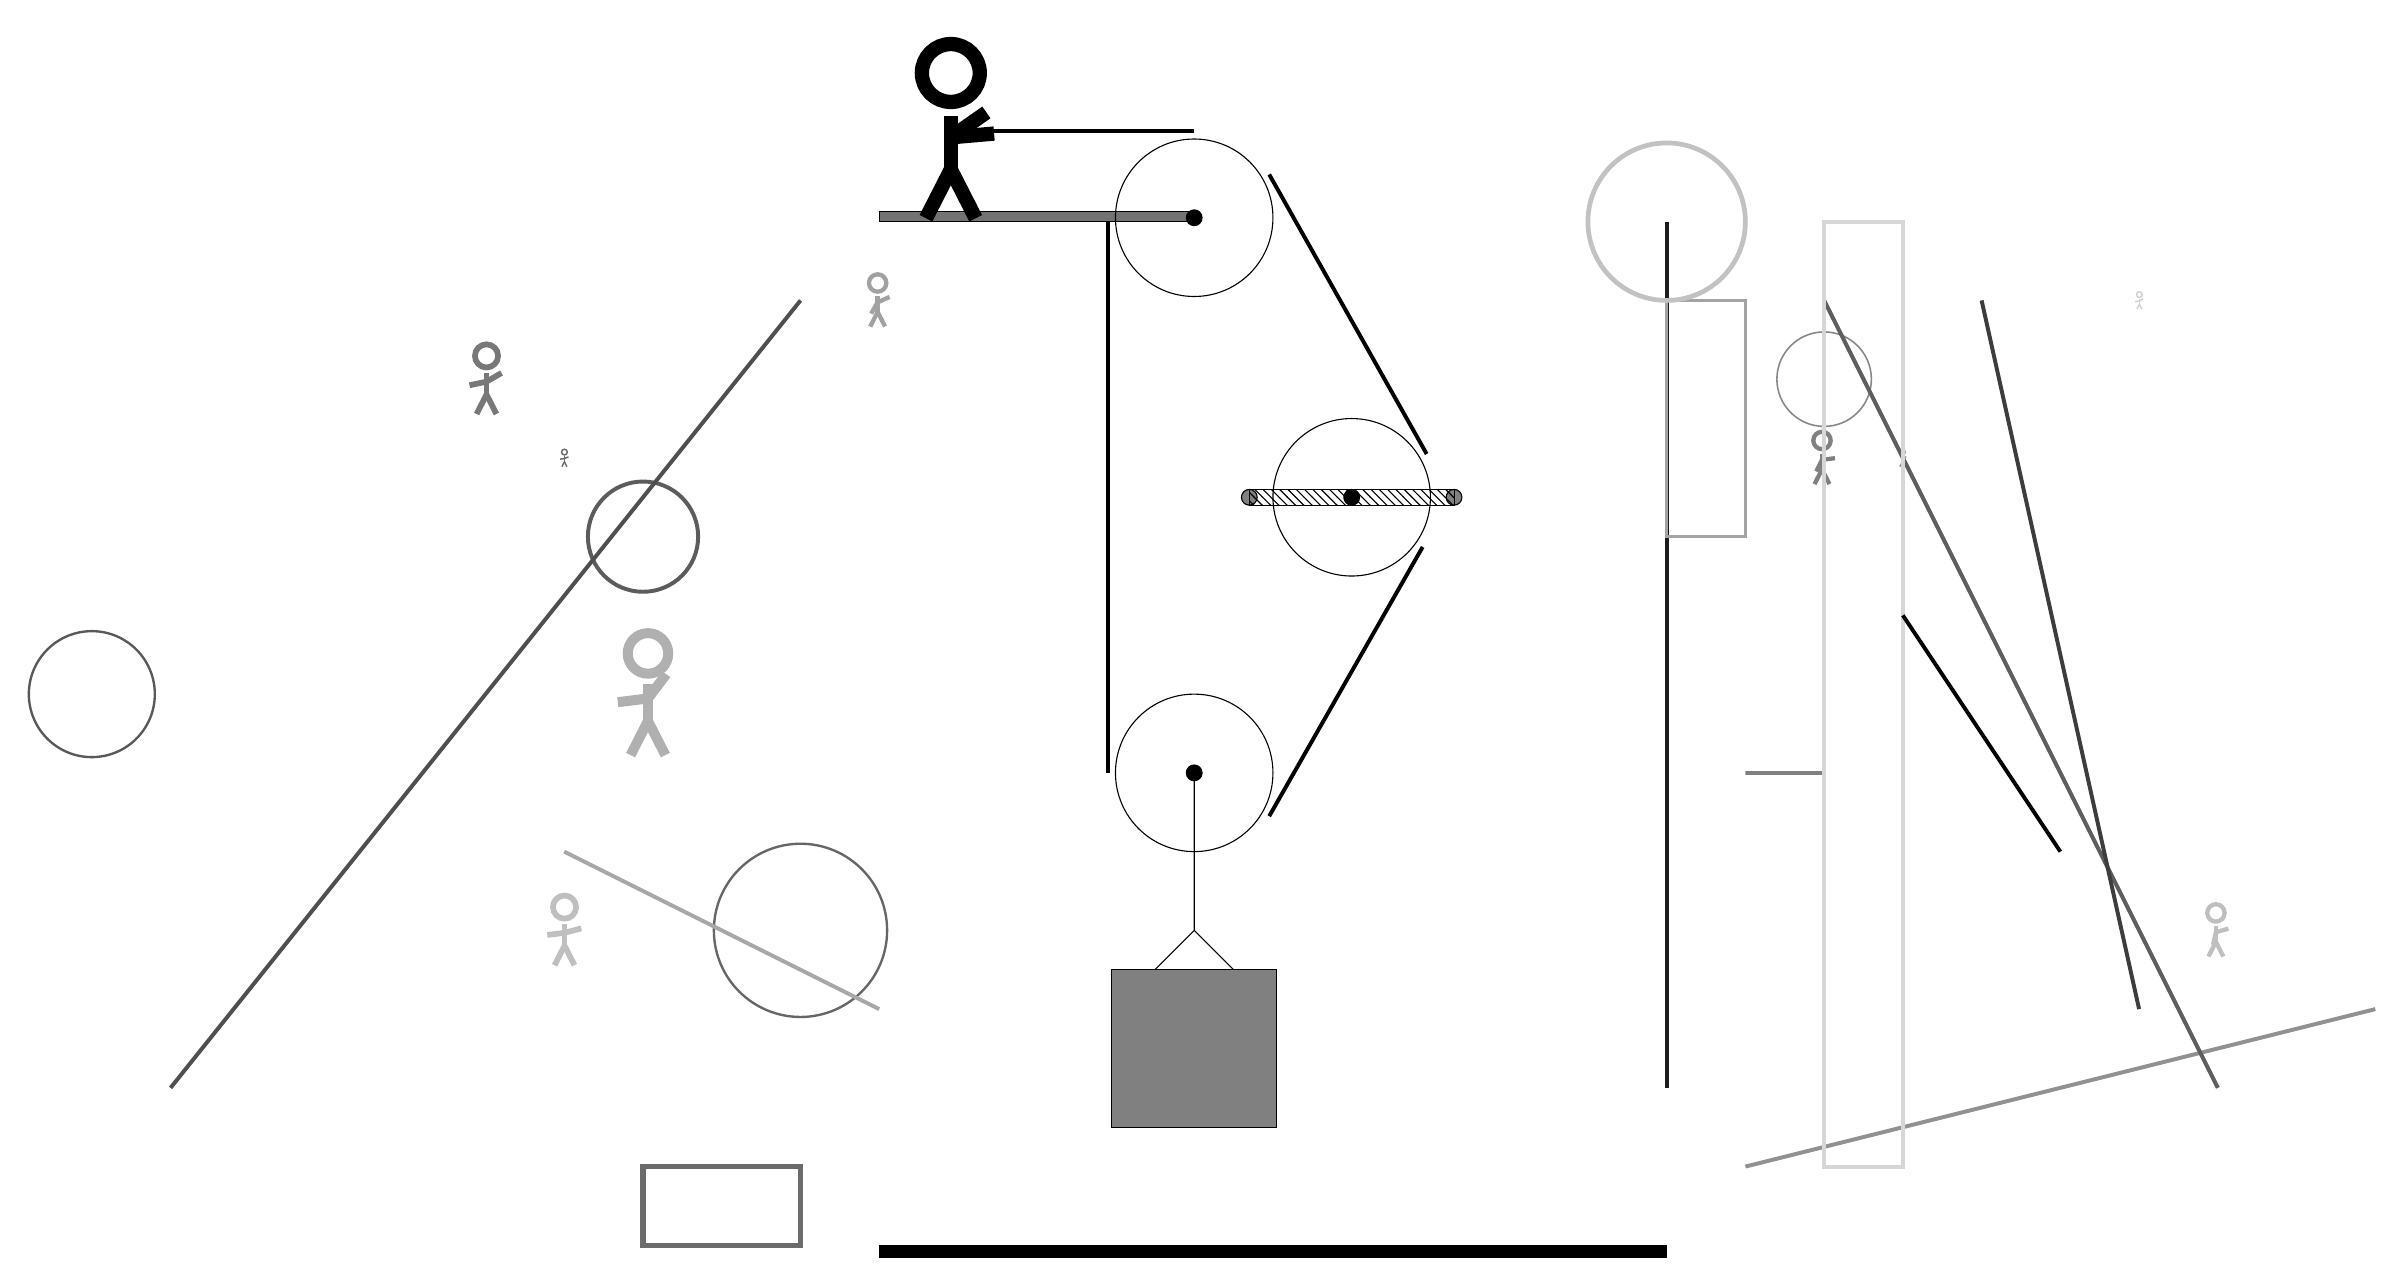
\begin{tikzpicture}
			%%%%% START %%%%%
			
			\draw[fill=black!55] (-2, 10) rectangle (2, 10.125);
			
			\draw (2, 3.0) circle (1);
			\draw[fill=black] (2, 3.0) circle (0.1);
			
			\draw (2, 10.05) circle (1);
			\draw[fill=black] (2, 10.05) circle (0.1);
			
			\draw[fill=white](4, 6.5) circle (1);
			\draw[fill=black] (4, 6.5) circle (0.1);
			\draw[fill=black!50] (2.7, 6.5) circle (0.1);
			\draw[fill=black!50] (5.3, 6.5) circle (0.1);
			\draw[pattern=north west lines, pattern color=black] (2.7, 6.6) rectangle (5.3, 6.4);
			
			\draw (2, 3.0) -- (2, 1.0) -- (1.5, 0.5) -- (2.5, 0.5) -- (2, 1.0);
			\draw[fill=black!50] (0.95, 0.5) rectangle (3.05, -1.5);
			
			\node[line width=0.3mm, color=black!43] at (11, 7) {\Strichmaxerl[1][82][23]};
			
			\node[line width=0.5mm, color=black!18] at (14, 9) {\Strichmaxerl[1][7][31]};
			\draw [line width=0.3mm, color=black!65](-12, 4) circle (0.8);
			\node[line width=0.4mm, color=black!59] at (-6, 7) {\Strichmaxerl[1][8][22]};
			\draw[line width=0.5mm, color=black!89](8, 10) -- (8, -1);
			\draw[line width=0.5mm, color=black!15] (10, 6) rectangle (10, 4);
			\draw[line width=0.4mm, color=black!36] (9, 9) rectangle (8, 6);
			\draw[line width=0.7mm, color=black!58] (-3, -3) rectangle (-5, -2);
			\node[line width=0.5mm, color=black!50] at (10, 7) {\Strichmaxerl[3][64][7]};
			
			\node[line width=0.2mm, color=black!25] at (15, 1) {\Strichmaxerl[3][77][16]};
			\draw [line width=0.5mm, color=black!64](-5, 6) circle (0.7);
			\draw[line width=0.5mm, color=black!43](9, -2) -- (17, 0);
			\draw[line width=0.6mm, color=black!50] (10, 3) rectangle (9, 3);
			\draw [line width=0.2mm, color=black!47](10, 8) circle (0.6);
			\draw [line width=0.3mm, color=black!60](-3, 1) circle (1.1);
			\draw[line width=0.5mm, color=black!63](10, 9) -- (15, -1);
			
			\node[line width=0.5mm, color=black!31] at (-5, 4) {\Strichmaxerl[7][7][53]};
			\node[line width=0.4mm, color=black!25] at (-6, 1) {\Strichmaxerl[4][7][15]};
			\draw[line width=0.5mm, color=black!16] (10, 10) rectangle (11, -2);
			\draw[line width=0.5mm, color=black!100](11, 5) -- (13, 2);
			\draw[line width=0.5mm, color=black!76](12, 9) -- (14, 0);
			
			\draw [line width=0.6mm, color=black!24](8, 10) circle (1.0);
			\node[line width=0.6mm, color=black!37] at (-2, 9) {\Strichmaxerl[3][60][24]};
			\draw[line width=0.5mm, color=black!34](-6, 2) -- (-2, 0);
			\draw[line width=0.5mm, color=black!69](-3, 9) -- (-11, -1);
			\node[line width=0.5mm, color=black!53] at (-7, 8) {\Strichmaxerl[4][12][30]};
			
			
			\draw[line width=0.5mm] (0.9, 10) -- (0.9, 3.0);
			\centerarc[line width=0.5mm](2, 3.0)(180:330:1.1);
			\draw[line width=0.5mm](2.9526, 2.45) -- (4.9011, 5.869);
			\centerarc[line width=0.5mm](4, 6.5)(390:325:1.1);
			\draw[line width=0.5mm](4.9526, 7.05) -- (2.9526, 10.6);
			\centerarc[line width=0.5mm](2, 10.05)(30:90:1.1);
			\draw[line width=0.5mm](2, 11.15) -- (-1, 11.15);
			
			\node at (-1, 11.15) {\Strichmaxerl[10][-175][35]};
			
			\draw[fill=black] (-2, -3) rectangle (8, -3.15);
			
			%%%%% END %%%%%
		\end{tikzpicture}
	\end{figure}	
\end{document}